\lecture{2}{Wed 29 May 2024 20:38}{Arithmetic with numbers}

\begin{definition}
    A natural number is a string of 1's:
    \[
        1,11,111,1111,11111,111111,1111111, \ldots
    .\]
\end{definition}


\begin{figure}[ht]
    \centering
    \incfig[1]{buffalos-and-antilops}
    \caption{Buffaloes and antilopes}
    \label{fig:buffaloes-and-antilopes}
\end{figure}

Now let's go back in time 1000000 years and imagine a person counting buffaloes and antilopes.
The figure represents buffaloes (squares) and antilopes (triangles).

Number of squares: 11111111111

Number of triangles: 11111111111

Total: 11111111111111111111111111

\begin{definition}
    The sum of numbers n and m is the combination of the strings of 1's. It is
    written n+m.
\end{definition}

\section*{Laws of addition}
\begin{itemize}
    \item n + m = m + n (commmunative) \hspace{10} 1111 + 111 = 111 + 1111
    \item (k + n) + m = k + (n + m) (associative) \hspace{10} (11 + 111) + 1111 = 11 + (111 + 1111)
    \item n + 1 = s (n) (succesor) \hspace{10}
\end{itemize}

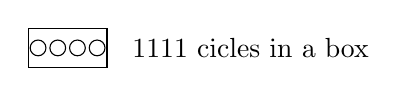
\begin{tikzpicture}
    % Draw the box with dimensions 0.5x1 cm
    \draw (0, 0) rectangle (1, 0.5);

    % Draw the circles with radius 0.1 cm
    \foreach \x in {0.125, 0.375, 0.625, 0.875} {
        \draw (\x, 0.25) circle [radius=0.1];
    }

    % Add a comment to the right side of the figure
    \node[right] at (1.2, 0.25) {1111 cicles in a box};
\end{tikzpicture}

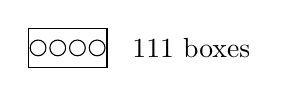
\begin{tikzpicture}
    % Draw the box with dimensions 0.5x1 cm
    \draw (0, 0) rectangle (1, 0.5);

    % Draw the circles with radius 0.1 cm
    \foreach \x in {0.125, 0.375, 0.625, 0.875} {
        \draw (\x, 0.25) circle [radius=0.1];
    }

    % Add a comment to the right side of the figure
    \node[right] at (1.2, 0.25) {111 boxes};
\end{tikzpicture}

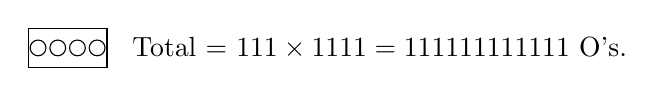
\begin{tikzpicture}
    % Draw the box with dimensions 0.5x1 cm
    \draw (0, 0) rectangle (1, 0.5);

    % Draw the circles with radius 0.1 cm
    \foreach \x in {0.125, 0.375, 0.625, 0.875} {
        \draw (\x, 0.25) circle [radius=0.1];
    }

    % Add a comment to the right side of the figure
    \node[right] at (1.2, 0.25) {Total = \( 111 \times 1111 = 111111111111\) O's.};
\end{tikzpicture}

\begin{definition}[Product]
    The product of numbers n and m is the string formed by a copy of m for every
    1 in n. It is written \( n \times m \).
\end{definition}

\section*{Laws of multiplication}
\begin{itemize}
    \item \( n \times m = m \times n  \) (commmunative)
    \item \((k \times n) \times m = k \times (n \times m) \) (associative)
    \item \( n \times 1 = n  \) (identity)
\end{itemize}

\section*{Distributive laws}
\begin{itemize}
    \item \( k \times (n + m) = (k \times n) + (k \times m) = k \times n + k \times m \)
    \item \( (k + n) \times m = k \times m + n \times m \)
\end{itemize}
